% !TeX document-id = {3aec7d78-4a32-4a0f-a5ca-01214b5f7293}
% +---------------------------------------------------------------+
% | Author :    Noémie Plancherel, HEIG-VD
% | Date :      04.03.22
% +---------------------------------------------------------------+

\documentclass[a4paper,11pt,twoside,openright]{book} % Type du document

% compiler avec : pdflatex, bibtex, pdflatex, pdflatex
% !TeX TXS-program:compile = txs:///pdflatex/[--shell-escape]


% +---------------------------------------------------------------+
% | Language
% +---------------------------------------------------------------+
\usepackage[T1]{fontenc}
\usepackage[utf8]{inputenc}
\usepackage[french]{babel}

\newif\ifisconfidential	\isconfidentialfalse

\newif\ifisdraft\isdraftfalse



% +---------------------------------------------------------------+
% | Paramètres
% +---------------------------------------------------------------+

\newcommand{\TBtitle}{Gestionnaires de mots de passe : quelle sécurité ? }
\newcommand{\TBsubtitle}{}%laisser vide si pas de sous-titre
\newcommand{\TByear}{2022}
\newcommand{\TBacademicYears}{2021-2022}

\newcommand{\TBdpt}{Département des Technologie de l'information et de la communication (TIC)}
\newcommand{\TBfiliere}{Filière Télécommunications}
\newcommand{\TBorient}{Orientation Sécurité de l'information}

\newcommand{\TBauthor}{Noémie Plancherel}
\newcommand{\TBsupervisor}{Prof. Sylvain Pasini}

% Confidentiel?
% uncomment if confidential / comment if not confiential
% \isconfidentialtrue

\newcommand{\TBresumePubliable}{
Dans ce travail... Ceci est le résumé publiable...
}

% +---------------------------------------------------------------+



% +-[set path]-------------------------------------+
\usepackage{template/TB-style}
\usepackage{template/TB-macros}
\usepackage{template/TB-template}
%\graphicspath{images/}


\begin{document}

\frontmatter
\pagestyle{empty}

% TITLE and template
% +---------------------------------------------------------------+

\TBmaketitle

\pagestyle{frontmatter}

\TBsecondTitle

\TBpreambule

\TBauthentification


% Cahier des charges
% +---------------------------------------------------------------+
% +---------------------------------------------------------------+
% | Author :    Noémie Plancherel, HEIG-VD
% | Date :      April 1st, 2022
% +---------------------------------------------------------------+


\chapter{Cahier des charges}



\section*{Résumé du problème}
De nos jours, les gestionnaires de mots de passe sont des outils très fréquemment utilisés. En effet, une bonne pratique est d'utiliser un mot de passe par service. De cette manière, si un service est compromis et le mot de passe divulgué, cela n'implique pas les autres. Il est également très important de choisir un mot de passe fort qui ne contient pas d'éléments facilement prévisibles et qui pourrait être brute-forcé rapidement. 

Les gestionnaires de mots de passe permettent principalement de faciliter le stockage des mots de passe qui demandent d'être de plus en plus longs et complexes, de manière à ne pas les réutiliser. Ils permettent également d'ajouter une couche sécuritaire aux mots de passe en les stockant de manière sécurisée et en offrant la possibilité de générer des mots de passe forts.

Ces applications offrent plusieurs fonctionnalités sous la forme de différents types;  elles permettent, entre autres, l'utilisation du cloud afin de stocker les mots de passe sur les serveurs du fournisseur pour faciliter la synchronisation des données entre plusieurs devices (mobile, montre, navigateur, etc.). Certains gestionnaires de mots de passe sont également fréquemment utilisés au sein d'entreprises pour permettre le partage de données. Les entreprises vont généralement utiliser une solution self-hosted où ils auront leur propre infrastructure et stockage. Il existe des extensions de navigateur  qui proposent le remplissage automatique de mots de passe dans les formulaires de connexion. Enfin, il y a également des applications en local qui vont limiter leur utilisation à un seul appareil.

Étant donné que les utilisateurs se reposent grandement sur les gestionnaires de mots de passe, il est important de s'assurer que ces logiciels satisfassent un certain nombre de principes de sécurité ainsi qu'une implémentation robuste afin d'éviter tout vol ou perte de données. 

\section*{Objectifs}
Ce travail de bachelor vise à comprendre les menaces d'un gestionnaire de mots de passe, premièrement de manière générique, puis sur des produits spécifiques, sélectionnés à la suite d'une étude complète, en analysant la sécurité sous différents angles (stockage, mémoire, réseau, cryptographie, etc.). 

Il est réalisé en deux parties distinctes; une première partie qui est une étude approfondie et complète sur les gestionnaires de mots de passe. Elle permet d'analyser les menaces des différents type de gestionnaires de mots de passe et de présenter les exigences sécuritaires qu'il serait nécessaire de garantir. Elle va également se concentrer sur une étude de marché avec une comparaison de plusieurs gestionnaires de mots de passe existants sous différents aspects.

La deuxième partie du travail se concentrera tout d'abord sur la sélection de quelques candidats (environ 4) en fonction de critères établis au préalable. Ensuite, le but est d'évaluer la sécurité de manière complète de chaque gestionnaire de mot de passe sélectionné; chaque élément choisi est analysé et évalué en fonction de différents critères comme les choix cryptographiques utilisés, le stockage, ou encore l'architecture de l'application.

%\begin{enumerate}
%	\item cloud
%	\item local - application desktop
%	\item extension de navigateur
%	\item closed-source
%\end{enumerate}

\subsection*{Livrables}
Les délivrables seront les suivants :
\begin{enumerate}
\item Une documentation contenant :
	\begin{itemize}
	\item Présentation des différents types de gestionnaires de mots de passe
	\item Étude de marché
	\item Une analyse de menaces de différents types de gestionnaires de mots de passe
	\item Spécification des exigences sécuritaires à garantir
	\end{itemize}
\item Analyse sécuritaire des quelques candidats représentatifs (environ 4) :
	\begin{itemize}
	\item Sélection de candidats pour la suite du travail
	\end{itemize}
chaque analyse se décomposera ainsi :
	\begin{itemize}
		\item Sélection de critères d'analyse
		\item Analyse complète de chaque aspect
		\item Rapport des faiblesses trouvées au fabricant
	\end{itemize}
\item Synthèse des résultats
\item Comparaison entre chaque candidat
\end{enumerate}

\subsection*{Déroulement}
En se référant aux dates officielles émises par la HEIG-VD, le travail de bachelor débute le 21 février 2022 et se termine au plus tard le 16 septembre 2022. Il y a 3 dates clés incluant des rendus:
\begin{itemize}
	\item \textbf{16 mai 2022} - rendu du rapport intermédiaire
	\item \textbf{29 juillet 2022} - rendu du rapport final
	\item \textbf{22 août au 16 septembre 2022} - soutenance du travail de bachelor
\end{itemize}

Etant donné, que la soutenance du travail implique l'intervention d'un expert, la date doit être définie entre tous les intervenants.

Le volume du travail de bachelor est de 15 crédit ECTS, soit 450 heures. Le rapport intermédiaire représente 150 heures de travail. Au niveau de la répartition de la charge de travail, cela représente ~13h/semaine jusqu'au 19 juin, puis 45h/semaine jusqu'au rendu, soit le 29 juillet. 




% TOC
% +---------------------------------------------------------------+
\tableofcontents
\clearpage


% Content
% +---------------------------------------------------------------+

\mainmatter
\pagestyle{plain}

% +---------------------------------------------------------------+
% | Author :    Noémie Plancherel, HEIG-VD
% | Date :      18.04.2022
% +---------------------------------------------------------------+


\chapter{Introduction}
\label{ch:intro}

Pour un utilisateur lambda, il peut être difficile de se souvenir de tous ses mots de passe tout en s'assurant d'en utiliser un différent pour chaque service afin d'éviter tout vol de données. Typiquement dans ces situations, nous allons naturellement utiliser des mots de passe simples, qui sont facilement mémorisables. Comme, par exemple, utiliser son prénom et sa date de naissance, "123456" ou encore "qwerty". De plus, il est plus simple d'utiliser le même mot de passe pour chacun de ses comptes, afin d'en mémoriser uniquement un seul. 

Cependant, même si l'unique mot de passe qu'on utilise est fort et aléatoire, il n'est pas garanti à 100\% qu'on soit la cible d'aucun attaquant et si une attaque est réalisée, toutes nos données personnelles sont exposées.

Ainsi, dans ce genre de cas, les gestionnaires de mots de passe interviennent et peuvent faciliter le quotidien de la plupart des utilisateurs. 

\section{Fonctionnement général}

Les gestionnaires de mots de passe sont des applications multi-plateformes qui vont permettre de stocker des informations sensibles telles que des mots de passe, numéros de carte de crédit ou encore des fichiers confidentiels. On peut les comparer à des coffres forts.  

Ces derniers proposent un \textit{master password} ou une \textit{master key} qui va permettre d'accéder à l'ensemble des données secrètes. En conséquence, la sécurité repose sur un seul mot de passe principal, ce qui est très bénéfique pour les utilisateurs car ils n'ont qu'un mot de passe à retenir. Une fois l'accès à l'application, l'utilisateur a la possibilité de stocker des données, générer des mots de passe ainsi que se connecter à des services en ligne (remplissage de formulaire d'identification automatique).

Les gestionnaires de mots de passe sont disponibles en plusieurs types différents en fonction du besoin de l'utilisateur et des fonctionnalités proposées. 

\section{Types}

\subsection{Cloud}
Les gestionnaires de mots de passe dans le cloud sont proposés pour un usage personnel ainsi qu'un usage professionnel. Les mots de passe entrés dans le coffre fort vont directement être stockés sur les serveurs du constructeur et ils seront également chiffrés sur ces derniers. Aucun stockage n'est effectué en local.

Le cloud va permettre aux utilisateurs d'avoir accès à leurs données sur n'importe quel device (ordinateur, mobile, montre) et à tout moment. De plus, toutes les données vont être synchronisées sur tous les devices connectés.

À propos de la sécurité, elle repose entièrement sur le provider de l'application car toutes les informations sont stockées sur leurs propres serveurs.

\subsection{Local}
Les applications en local s'installent sur le desktop ou sur le mobile de l'utilisateur. Ces gestionnaires de mots de passe fonctionnent indépendamment et sont offline. Ces produits peuvent donc être utilisés sur une seule machine, par conséquence la synchronisation n'est pas proposée pour ce type de password manager. 

Toutes les données sensibles sont directement stockées et chiffrées sur le device. La sécurité est plutôt bonne comparé à la solution cloud car c'est du hors-ligne, cependant si on récupère / vole le device, la sécurité devient plus faible car il y aurait la possibilité d'avoir accès aux informations sensibles du gestionnaire de mots de passe, via notamment une gestion de mémoire mal gérée. 

Il y a également une solution \textit{on-premise} (ou \textit{self-host}) qui permet d'utiliser sa propre infrastructure locale pour héberger toutes les données du gestionnaire de mots de passe. Les fonctionnalités offertes sont les mêmes que pour les solutions cloud mais le prix est en général plus cher et l'application plus orientée professionnelle.

\subsection{Navigateur}
Le dernier type de gestionnaire de mots de passe sont ceux qui sont basés sur le navigateur (\textit{browser-based}). Les navigateurs les plus populaires, tels que Firefox, Safari ou Chrome offrent ce gestionnaire de mots de passe qui est directement inclu dans ces derniers.
Ils vont faciliter la gestion et la sauvegarde de mots de passe de comptes de sites web. Il y a également la possibilité de synchroniser toutes les données stockées entre tous les devices qui supportent le navigateur en question (Chrome, Firefox, Safari, etc.).

Pour certains navigateurs, les informations sont stockées et chiffrées en local sur le device de l'utilisateur. Si la synchronisation est activée, les données seront également stockées dans le cloud sur les serveurs du constructeur. Un problème de sécurité importante, et la disponibilité des mots de passe sur le navigateur, si aucun master password n'est configuré et qu'on a accès à la machine, les mots de passe sont accessibles en clair sur le navigateur.


% +---------------------------------------------------------------+
% | Author :    Sylvain Pasini, HEIG-VD
% | Date :       June 3rd, 2021
% +---------------------------------------------------------------+


\chapter{État de l'art}
\label{ch:etatdelart}


%exemple
\lipsum[1-4]



% +---------------------------------------------------------------+
% | Author :    Sylvain Pasini, HEIG-VD
% | Date :       June 3rd, 2021
% +---------------------------------------------------------------+


\chapter{Exemple de chapitre}

\lipsum[1]


\section{math}

voici des maths intégrés : $3^2 / 4^3$.

ou alors à la ligne :

$$ \frac{3 x_a}{ y_b^2 +4}$$

\section{images ?}

Voici comment mettre une image.

\begin{figure}
	\centering
	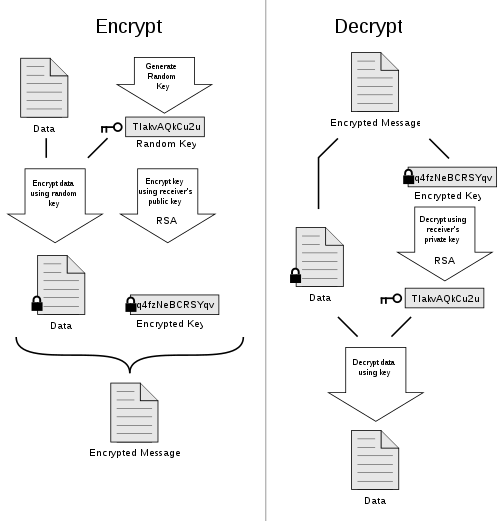
\includegraphics[width=8cm]{images/PGP_101.png}
	\caption{Schéma PGP}
	\label{fig:pgp}
\end{figure}


\section{comment citer une référence bibliographique ?}

Ceci est un exemple de citation d'un livre de Pasini~\cite{pasini2015}.

Mais aussi du site Web de Black Alps 2019~\cite{BA19} !


\section{comment faire une référence ?}

On peut aussi ajouter une référence à la section~\ref{sec:shell}.

On peut aussi ajouter une référence à l'introduction, chapitre~\ref{ch:intro}.

Comme montre la Figure~\ref{fig:pgp}, on peut référencer une figure.


\section{comment afficher une commande simple ou du bash}

Utiliser la commande \com{com}.

Exemple : Test d'une commande bash shell \com{ls} : 

Utiliser l'environnement \com{shellcmd}.

\begin{shellcmd}
$> ls -al test_underscore $$* "coucou"
\end{shellcmd}
Bli bLa


\section{Commande Shell}
\label{sec:shell}

Voici comment faire une mise en forme de commande SHELL.

Utiliser l'environnement \com{listingsbox}.
\begin{description}
 \item[1er paramètre:] le ype de shell, ici "console"
 \item[2ème paramètre:] le nom à donner à la box
\end{description}

\begin{listingsbox}{console}{Exemple de commande shell avec réponse}
root@kali:~$ bunzip2 data-decrypted.bin
bunzip2: Can't guess original name for data-decrypted.bin -- using
data-decrypted.bin.out
\end{listingsbox}


\section{Code inclus en direct dans le latex}

Utiliser l'environnement \com{sourcebox}.
\begin{description}
 \item[1er paramètre:] le ype de shell, ici "c"
 \item[2ème paramètre:] le nom à donner à la box
\end{description}

\begin{sourcebox}{c}{Exemple de code C}
#include <stdio.h>

int main(int argc, char* argv[])
{
   printf("Hello World!\n");
   return 0;
}
\end{sourcebox}



\section{Code à partir d'un fichier}

Utiliser la commande \com{inputsourcecode}.
\begin{description}
 \item[1er paramètre:] le ype de shell, ici "c"
 \item[2ème paramètre:] le nom du fichier source, "\path{source_code/example.c}"\\ Egalement exemple de la commande \com{path}.
 \item[3ème paramètre:] le nom à donner à la box
\end{description}


%% Inclure du code source d'un fichier externe
%% 1er paramètre: langage du code
%% 2ème paramètre: le path du fichier source
%% 3ème paramètre: le titre de la box
\inputsourcecode{c}{"source_code/example.c"}{Fichier complet example.c}

Même exemple, mais en spécifiant les lignes 4 à 8 :
\inputsourcecode[firstline=4,lastline=8]{c}{"source_code/example.c"}{Lignes 4 à 8 de example.c}





% +---------------------------------------------------------------+
% | Author :    Sylvain Pasini, HEIG-VD
% | Date :       June 3rd, 2021
% +---------------------------------------------------------------+


\chapter{Architecture}
\label{ch:arch}


%exemple
\lipsum[1-4]



% +---------------------------------------------------------------+
% | Author :    Sylvain Pasini, HEIG-VD
% | Date :       June 3rd, 2021
% +---------------------------------------------------------------+


\chapter{Implementation}
\label{ch:impl}


%exemple
\lipsum[1-4]



% +---------------------------------------------------------------+
% | Author :    Sylvain Pasini, HEIG-VD
% | Date :       June 3rd, 2021
% +---------------------------------------------------------------+


\chapter{Conclusion}



% +---------------------------------------------------------------+
%\backmatter

\cleardoublepage
\phantomsection
\addcontentsline{toc}{chapter}{Bibliographie}
\bibliographystyle{plain}
\bibliography{chapters/biblio}
\nocite{*} %ajoute tout ce qu'il y a dans le bibtex

\cleardoublepage
\phantomsection
\addcontentsline{toc}{chapter}{Liste des figures}
\listoffigures

\cleardoublepage
\phantomsection
\addcontentsline{toc}{chapter}{Liste des tableaux}
\listoftables

\cleardoublepage
\phantomsection
\addcontentsline{toc}{chapter}{Liste des listings}
%\listoflistings
\tcblistof[{\chapter*}]{mypyg}{Liste des listings}


% Annexes
% +---------------------------------------------------------------+
\appendix

% +---------------------------------------------------------------+
% | Author :    Sylvain Pasini, HEIG-VD
% | Date :       June 3rd, 2021
% +---------------------------------------------------------------+


\chapter{Outils utilisés pour la compilation}

%exemple
\lipsum[5-6]


% +---------------------------------------------------------------+
% | Author :    Sylvain Pasini, HEIG-VD
% | Date :       June 3rd, 2021
% +---------------------------------------------------------------+


\chapter{Journal de travail}

\begin{landscape}

\begin{longtable}[c]{lp{10cm}rrrr}
    \caption{Journal de travail}\\

    \hline
    Date & Description & Rech. [h] & Dev. [h] & Rapport [h] & Admin [h] \\
    \hline
    \endfirsthead
    
    \hline
    Date & Description & Rech. [h] & Dev. [h] & Rapport [h] & Admin [h] \\
    \hline
    \endhead
    
    \multicolumn{6}{r}{\small \it Le journal de travail continue à la page suivante.} \\
    \normalsize
    \endfoot
    
    \hline
    \endlastfoot


  % Work
    > 20.09.22
    & Discussion avec le professeur responsable, établissement du cahier des charges, introduction
    & 7 %recherche
    & 0 %dev
    & 10 %reporting
    & 4\\ %admin
    
	20.09.2022 
	& Update + organisation du TB, planing, relire le début du TB déjà commencé, avancement de l’étude du marché (fonctionnalités, plateformes, prix), lecture d’articles
	& 2 %recherche
	& 0 %dev
	& 5 %reporting
	& 1\\ %admin

	21.09.2022 
	& Recherches sur les statistiques des gestionnaires de mots de passe sur le marché, rédaction du chapitre étude de marché (terminé ce jour-ci)
	& 3 %recherche
	& 0 %dev
	& 3 %reporting
	& 0\\ %admin

	22.09.2022
	& Introduction et organisation du chapitre étude sécuritaire, recherche et lecture sur les différentes implémentations sécuritaire des gestionnaires de mots de passe
	& 3 %recherche
	& 0 %dev
	& 1 %reporting
	& 1\\ %admin

	23.09.2022 
	& Recherche et lecture sur les différentes implémentations sécuritaire des gestionnaires de mots de passe et organisation du rapport
	& 1 %recherche
	& 0 %dev
	& 1 %reporting
	& 0\\ %admin

	26.09.2022  
	& Recherche et lecture sur les gestionnaires de mots de passe browser-based, rédaction dans le rapport à ce propos
	& 4 %recherche
	& 0 %dev
	& 1 %reporting
	& 0\\ %admin
	
	
	27.09.2022  
	& Recherche et lecture sur les gestionnaires de mots de passe browser-based et local-based, et rédaction dans le rapport
	& 3 %recherche
	& 0 %dev
	& 2 %reporting
	& 0\\ %admin
	
	28.09.2022  
	& Recherche et lecture sur les gestionnaires de mots de passe browser-based et local-based, et rédaction dans le rapport
	& 4 %recherche
	& 0 %dev
	& 1 %reporting
	& 0\\ %admin

	29.09.2022  
	& Recherche et lecture sur les gestionnaires de mots de passe local-based, et rédaction dans le rapport
	& 5 %recherche
	& 0 %dev
	& 3 %reporting
	& 0\\ %admin

	30.09.2022 
	& Rédaction de la section du partage d'informations, des 3 états du gestionnaires de mots de passe 
	& 1 %recherche
	& 0 %dev
	& 4 %reporting
	& 0\\ %admin

	03.10.2022 
	& Fin du chapitre 3 sur analyse de menaces, lecture sur la modélisation de menaces et la norme que je souhaite suivre
	& 7 %recherche
	& 0 %dev
	& 1 %reporting
	& 0\\ %admin

	04.10.2022
	& Début chapitre analyse de menaces et lecture de la norme choisie
	& 6 %recherche
	& 0 %dev
	& 2 %reporting
	& 0\\ %admin
	
	05.10.2022
	& Lecture et rédaction établissement du contexte de l'analyse de menaces
	& 5 %recherche
	& 0 %dev
	& 3 %reporting
	& 0\\ %admin

	06.10.2022 
	& Lecture et rédaction établissement du contexte de l'analyse de menaces
	& 2 %recherche
	& 0 %dev
	& 6 %reporting
	& 0\\ %admin

	07.10.2022 
	& Lecture et rédaction identification des risques de l'analyse de menaces
	& 5 %recherche
	& 0 %dev
	& 3 %reporting
	& 0\\ %admin

	09.10.20220 
	& Lecture et rédaction identification des risques de l'analyse de menaces
	& 2 %recherche
	& 0 %dev
	& 2 %reporting
	& 0\\ %admin
	
	10.10.20220 
	& Lecture et rédaction identification des risques de l'analyse de menaces
	& 3 %recherche
	& 0 %dev
	& 5 %reporting
	& 0\\ %admin
	
	11.10.20220 
	& Rédaction et lecture analyses des risques et évaluation des risques
	& 4 %recherche
	& 0 %dev
	& 4 %reporting
	& 0\\ %admin
	
	12.10.20220 
	& Rédaction et lecture analyses des risques et évaluation des risques
	& 3 %recherche
	& 0 %dev
	& 4 %reporting
	& 0\\ %admin
	
	13.10.20220 
	& Rédaction du traitement des risques et lecture à ce propos avec les contremesures possibles
	& 3 %recherche
	& 0 %dev
	& 3 %reporting
	& 0\\ %admin
	
	14.10.20220 
	& Rédaction de la section exigences sécuritaires à respecter, relecture du TB, organisation du rapport et rendu intermédiaire du rapport
	& 1 %recherche
	& 0 %dev
	& 6 %reporting
	& 0\\ %admin

	16.10.20220
	& Rédaction de la sélection des candidats
	& 2 %recherche
	& 0 %dev
	& 6 %reporting
	& 0\\ %admin
	
\end{longtable}


\end{landscape}


\end{document}

% Auteur : Sylvain Pasini, HEIG-VD, 2021
